%% *ACL (ARR) submission, anonymous. Compile with pdflatex from the repository
%% root, exactly like main.tex:  pdflatex paper/main_acl.tex
%%
%% This wrapper shares every section file with the AAAI build (main.tex); only
%% the preamble and the back-matter ordering differ. Switch "review" to "final"
%% for the camera-ready, or to "preprint" for a non-anonymous arXiv version.
\documentclass[11pt]{article}
\usepackage[review]{acl}

%% Standard *ACL template includes
\usepackage{times}
\usepackage{latexsym}
\usepackage[T1]{fontenc}
\usepackage[utf8]{inputenc}
\usepackage{microtype}
\usepackage{inconsolata}
\usepackage{graphicx}

%% Packages this paper needs on top of the template.
%% NOTE: acl.sty already loads natbib, caption and hyperref. Do not load them
%% again here, or the citation and caption formatting will break.
\usepackage{booktabs}
\usepackage{multirow}
\usepackage{amsmath}
\usepackage{enumitem}
\usepackage{xspace}
\usepackage{tikz}
\usetikzlibrary{positioning, arrows.meta, calc}
\setcounter{secnumdepth}{2}

%% Portable check / cross (drawn, not font glyphs).
%% These MUST be robust: a TikZ picture is fragile, and hyperref (loaded by
%% acl.sty) expands caption text, which breaks an unprotected \tikz.
\DeclareRobustCommand{\cmark}{\tikz[baseline=-0.55ex]{\draw[green!55!black,line width=0.9pt] (0,0.6pt)--(2pt,-1.4pt)--(5pt,3.6pt);}}
\DeclareRobustCommand{\xmark}{\tikz[baseline=-0.55ex]{\draw[red!75!black,line width=0.9pt] (0,0)--(4pt,4pt) (0,4pt)--(4pt,0);}}
\DeclareRobustCommand{\checkmark}{\cmark}
\newcommand{\fininteract}{\textsc{FinInteract}\xspace}
\newcommand{\interactcomp}{\textsc{InteractComp}\xspace}
\newcommand{\HO}{$H_0$\xspace}
\newcommand{\disep}{$\text{DisE}^+$\xspace}
\newcommand{\disei}{$\text{DisE}^+$\xspace}

%% Where the shared appendix should point for the short limitations list.
%% *ACL puts it in an unnumbered \section*, which has no number to \ref.
\newcommand{\limref}{the Limitations section}

%% Venue code of ethics cited by the generative-AI disclosure in the appendix.
\newcommand{\ethicscode}{the ACL Code of Ethics}

\title{FinInteract: Benchmarking Clarification and Intent Integration in Ambiguous Financial Question Answering}

%% Under the "review" option acl.sty replaces this with "Anonymous ACL
%% submission". Fill in real authors before switching to "final".
\author{
  Anonymous ACL submission \\
}

\begin{document}
\maketitle

\begin{abstract}
%% Shared abstract body, inputted by both main.tex (AAAI) and main_acl.tex (*ACL).
Large language model agents are increasingly deployed for financial information retrieval, and hence for downstream analytics and investment decisions. However, financial terminology is highly specific, and a question without sufficient specification may admit multiple defensible readings with materially different values, e.g., Meta Platforms' ``operating income'' is \$46.75B consolidated or \$62.87B for the Family of Apps segment, while each reading's ground truth is exact and programmatically verifiable. A capable agent should recognize the ambiguity and ask a clarification question instead of committing to a plausible but unintended reading. Existing financial benchmarks cannot see this, because they attach only one gold answer per question and therefore fail to distinguish agents that resolve the ambiguity from those making ungrounded guesses, a blind spot we call the \emph{single-gold illusion}. To address this illusion, we release \fininteract, a bilingual (English/Chinese) benchmark of 173 instances that pairs each question with a \emph{default} and an \emph{intended} interpretation (fixed by a disambiguating context) across a five-category ambiguity taxonomy, and grades whether an agent elicits and then integrates the right clarification. Re-grading the \emph{same} retrieval-augmented outputs against the intended rather than the default reading cuts GPT-4o's measured accuracy by a factor of $3.1$ ($37.0\%$ to $12.1\%$), so a single-gold convention would have reported roughly three times the model's true competence. Our fine-grained analysis shows that this failure is one of interaction: models answer above $90\%$ correctly once the interpretation is supplied, but reach at most $28.9\%$ under their own clarification at full scale ($44.0\%$ in a cross-vendor pilot), so the bottleneck lies in issuing the correct clarification and then integrating the answer. We further report a skill metric that localizes failure modes of different financial ambiguities across two well-powered categories (entity scope and metric definition) and three exploratory ones.

\end{abstract}

%% ============================================================
\section{Introduction}
\label{sec:intro}
%% ============================================================
Large language model (LLM) agents are increasingly utilized in financial analysis to answer questions in regulatory filings~\citep{islam2023financebench,chen2021finqa,reddy2024docfinqa}, carry out multi-step research and retrieval over corporate disclosures~\citep{bigeard2025financeagent,choi2025finagentbench,krumdick2024bizbench,xie2024finben}. The agent reads a user's question, searches through relevant filings and returns the answer for downstream actions. 

However, financial questions are often deceptively under-specified. Financial terminology is highly specific, and a natural language question may map to several defensible readings for different numbers, e.g. in the question \emph{``What was Meta Platforms' operating income?''} (Figure~\ref{fig:teaser}), an agent must decide whether the user means the consolidated GAAP figure (\$46.75B for FY2023) or the Family of Apps segment (\$62.87B), both being programmatically verifiable against SEC facts. A capable agent should recognize the ambiguity and follow up with the user instead of directly committing into a plausible but unintended reading. 

Existing financial benchmarks cannot measure this as they grade only the final answer by assuming the question is disambiguated~\citep{islam2023financebench,chen2021finqa,reddy2024docfinqa,krumdick2024bizbench,xie2024finben}. Without grounding check, they cannot distinguish whether the agent actually resolves the ambiguity or guesses the common reading. We call such blind spot \emph{single-gold illusion} (Table~\ref{tab:comparison}), which is currently underexplored in the financial domain relative to general ambiguous QA literature~\citep{min2020ambigqa,li2025condambigqa,kuhn2022clam}. We study financial ambiguity over three research questions: \begin{itemize}[leftmargin=*, topsep=3pt, itemsep=1pt, parsep=0pt]
    \item \textbf{RQ1}: Do frontier models recognize financial report ambiguity? 
    \item \textbf{RQ2}: What financial ambiguity leads to most failures?
    \item \textbf{RQ3}: Can we incorporate interventions at inference time to improve resolution?
\end{itemize}

\begin{figure*}[t]
\centering
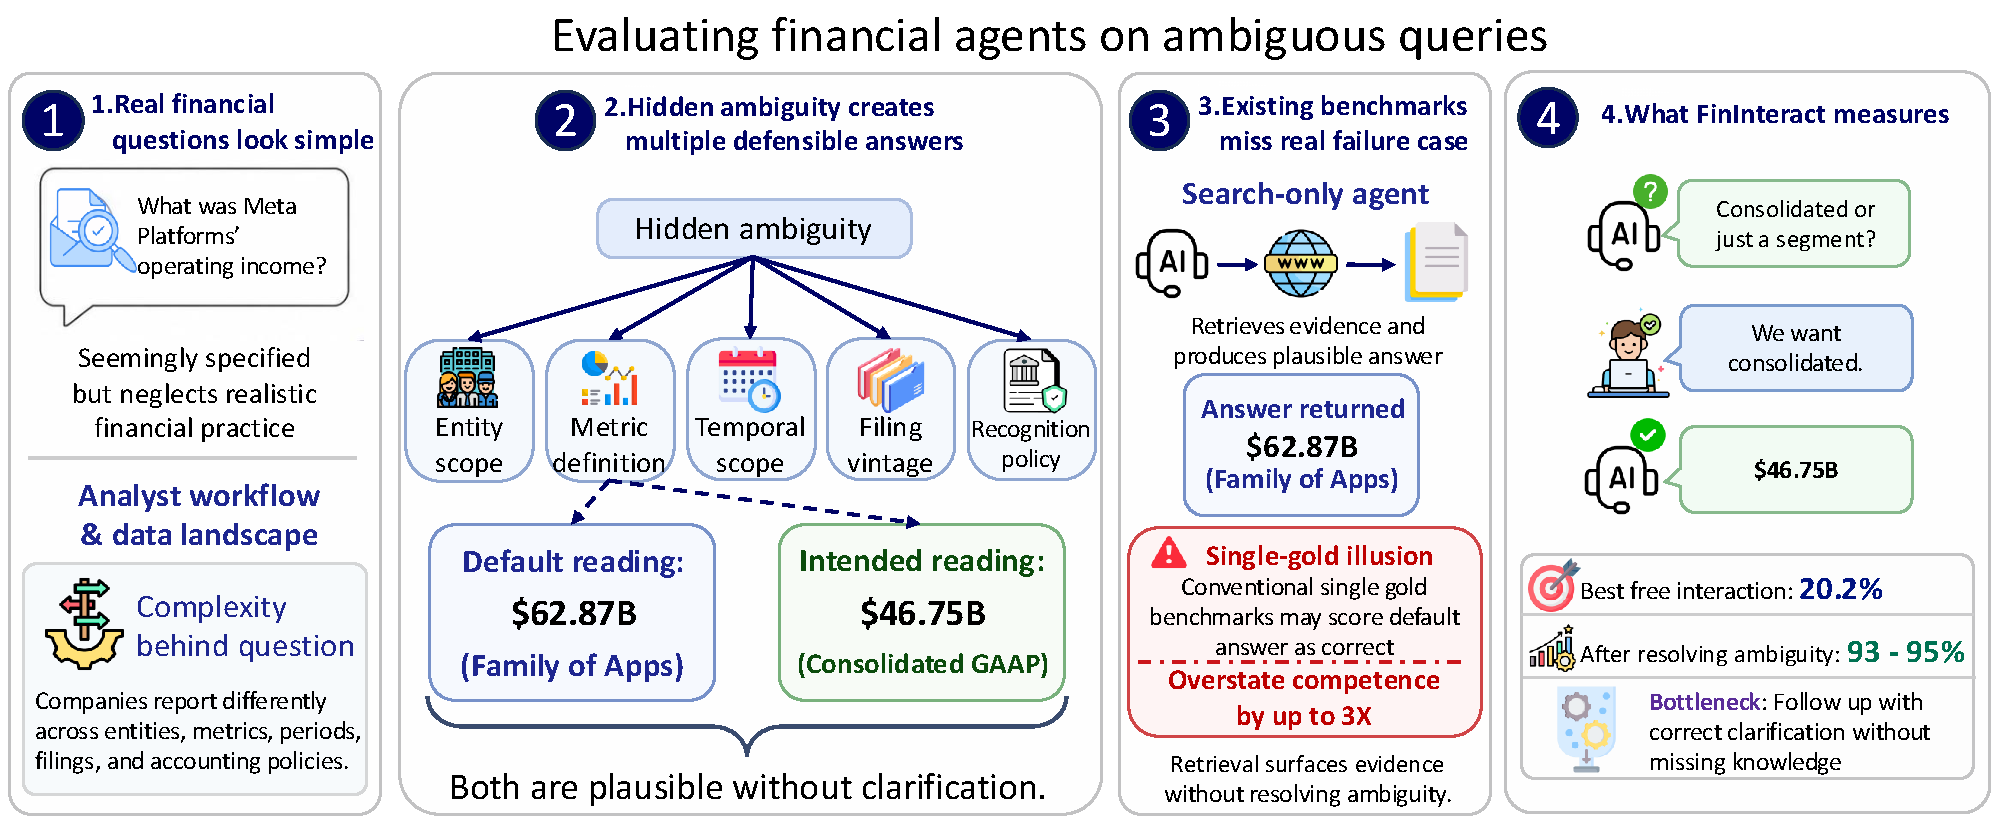
\includegraphics[width=\textwidth]{motivation_plot.pdf}
\caption{\textbf{Evaluating financial agents on ambiguous queries.}
\textbf{(1)}~A real analyst query (``What was Meta Platforms' operating income?'') looks
fully specified, but neglects that companies report differently across entities, metrics,
periods, filings, and accounting policies. \textbf{(2)}~The query hides ambiguity along five
categories (entity scope, metric definition, temporal scope, filing vintage, recognition policy),
here yielding two defensible answers, a default reading of \$62.87B (Family of Apps segment)
and the intended \$46.75B (consolidated GAAP), both plausible without clarification.
\textbf{(3)}~A search-only agent retrieves evidence and returns the plausible default, which
a conventional single-gold benchmark scores as correct, the \emph{single-gold illusion} that
overstates competence by up to $3\times$. \textbf{(4)}~\fininteract instead measures whether
an agent resolves the ambiguity by asking: for the GPT-5 agent shown, free-interaction
accuracy is $20.2\%$ while accuracy once the ambiguity is resolved is $93$--$95\%$, so the
bottleneck is issuing the right clarification without missing knowledge.}
\label{fig:teaser}
\end{figure*}

\begin{table}[h]
\centering
\caption{Running example: a \fininteract instance.
The paired default and intended readings are shown; $H_0{=}\log_2 3{\approx}1.58$ reflects
three plausible entity scopes for this question (consolidated total and two reportable
segments). Without the disambiguating context $C$, a model's default interpretation
leads to the wrong answer.}
\label{tab:example}
\small
\resizebox{0.9\columnwidth}{!}{%
\begin{tabular}{p{1.8cm}p{5.7cm}}
\toprule
Field & Value \\
\midrule
$Q$ &
  What was Meta Platforms' operating income? \\
$C$ &
  Total company (consolidated) results under U.S.\ GAAP for the year
  ended December 31, 2023. \\
$A$ (intended) &
  \$46.75B \emph{[consolidated GAAP]} \\
$A_d$ (default) &
  \$62.87B \emph{[Family of Apps segment]} \\
\midrule
Ambiguity category & Entity scope \\
$H_0$ & 1.58 bits \\
\midrule
Intended span &
  ``Income from operations for 2023 was \$46.75 billion\ldots'' \\
Default span &
  ``Family of Apps\ldots Income from operations \$62,871\ldots'' \\
\bottomrule
\end{tabular}}
\end{table}

Answering these questions requires three design properties. First,
the benchmark must draw representative ambiguity from real filings. Second, it must expose fine-grained dimensions of ambiguity through paired default and intended readings. Third, benchmark construction should have low cost and is safe from potential leakage to keep answer out of disambiguating context, with verifiable ground truth validated by domain experts. (Sec. \ref{sec:task}).

We release \fininteract, a bilingual benchmark in English and Chinese containing 173 instances, classified into five financial ambiguity categories. Each question $Q$ is paired with a \emph{default} interpretation recording a possible non-expert assumption and an \emph{intended} interpretation fixed by the disambiguating context. By grading the same model outputs against the default and intended interpretations, we effectively expose this single-gold illusion. \fininteract includes skill metric to localize which clarification ability the model lacks, and evaluates the agents under a ReAct protocol where the user simulator answers only from the disambiguating context (Figure~\ref{fig:framework}) to measure the agent's quality of clarify-then-integrate action. 

Our evaluation answers the research questions in turn. First, while frontier models detect ambiguity, they rarely resolve it effectively, as they ask the correct clarification question but still \textbf{failing to convert into the correct answer at the end} (Sec. \ref{sec:skills}). Second, \textbf{policy-related ambiguities} are the least resolved, as none of the proprietary models would initiate clarifications when facing this sparse category. Third, \textbf{inference intervention facilitates ambiguity resolution}, increasing accuracy from about 44\% to above 90\%, suggesting that this benchmark is not only diagnostic but also actionable. (Appendix~\ref{app:findings}). This paper makes three contributions \begin{enumerate}[leftmargin=*,itemsep=1pt]
  \item \textbf{Problem definition.} We formalize ambiguity in financial questions with five categories grounded in standard accounting and disclosure practice (Sec. \ref{sec:task}).
  \item \textbf{Benchmark.} We introduce \fininteract, a bilingual financial ambiguity dataset containing 173 instances, each paired with a default and an intended interpretation verified by domain experts. (Sec. \ref{sec:methodology}).
  \item \textbf{Empirical findings.} Our evaluation shows that existing models commonly fail to return correct final answer even when they have correctly clarified the intention, which can be improved via intervention at inference time. (Sec. \ref{sec:exp}).
\end{enumerate}


%% ============================================================
\section{Problem Formulation}
\label{sec:task}
%% ============================================================
Given an ambiguous financial question instance (example in Table~\ref{tab:example}), it should contain the ambiguous question over a company filing $Q$, the disambiguating context $C$ which is the minimal set of scope or definitional constraints that collapses $Q$ into the unique intended answer $A$ under intended interpretation $\mathcal{I}_{\text{int}}$. The ambiguous question typically contains correct answer $A_{d}\neq A$ under the default interpretation $\mathcal{I}_{\text{def}}$ which a non-expert would assume when reading $Q$. Specifically, $\mathcal{I}_{\text{int}},\mathcal{I}_{\text{def}}$ are structured records specifying the financial ambiguity taxonomy defined below. 
\begin{table}[h]
\centering
\caption{This example of ambiguous financial question contains three plausible entity scopes, i.e. consolidated total and two reportable segments, leading to an entropy of $1.58$ bits. Without the disambiguating context $C$, a model's default interpretation leads to the wrong answer.}
\label{tab:example}
\small
\begin{tabular}{p{2.7cm}p{4.7cm}}
\toprule
Field & Value \\
\midrule
$Q$ &
  What was Meta Platforms' operating income? \\
$C$ &
  Total company (consolidated) results under U.S.\ GAAP for the year
  ended December 31, 2023. \\
$A$ (intended) &
  \$46.75B \emph{[consolidated GAAP]} \\
$A_d$ (default) &
  \$62.87B \emph{[Family of Apps segment]} \\
\midrule
Ambiguity category & Entity scope \\
$H_0$ & 1.58 bits \\
\midrule
Intended span &
  ``Income from operations for 2023 was \$46.75 billion\ldots'' \\
Default span &
  ``Family of Apps\ldots Income from operations \$62,871\ldots'' \\
\bottomrule
\end{tabular}
\end{table}

\textbf{Financial ambiguity taxonomy.}
\label{sec:taxonomy}
We derive five categories of financial ambiguity from standard
accounting and disclosure practice (Table~\ref{tab:axes}). Each instance should normally exercise one primary category with one or two optional secondary categories in case of additional ambiguity. 

\begin{table}[h]
\centering
\caption{Five-category financial ambiguity taxonomy.}
\label{tab:axes}
\small
\begin{tabular}{p{2.0cm}p{5.5cm}}
\toprule
Category & Definition \\
\midrule
\textbf{Temporal scope} &
  Ambiguity over which time period is intended: fiscal year ending
  September vs. calendar year; Q3 results vs. full year; TTM vs.
  point-in-time. \\
\addlinespace
\textbf{Metric definition} &
  Ambiguity over accounting basis: GAAP net income vs. non-GAAP adjusted
  income; organic revenue vs. as-reported; operating EBITDA vs. net income. \\
\addlinespace
\textbf{Entity scope} &
  Ambiguity over consolidation level: segment vs. consolidated total;
  parent-attributable vs. full consolidated; Class A vs. Class B shares;
  A-shares vs. H-shares. \\
\addlinespace
\textbf{Filing vintage} &
  Ambiguity over filing version: original 10-K vs. amended 10-K/A;
  as-reported vs. restated; preliminary earnings release vs. final filing. \\
\addlinespace
\textbf{Recognition policy} &
  Ambiguity over accounting policy: revenue recognized point-in-time
  vs. over time; gross vs. net revenue; capitalized vs. expensed R\&D. \\
\bottomrule
\end{tabular}
\end{table}

\textbf{Disambiguation entropy.} We quantify how ambiguous an instance is using the prior confidence entropy $H_{0} = \log_{2} k$, where $k$ denotes the number of plausible interpretations of $Q$ without clarifying interaction, e.g. the example in Table~\ref{tab:example} has three plausible interpretations, hence contributing to an entropy of $H_0 = \log_2 3 \approx 1.58$ bits. This further serves as our metric to evaluate difficulty and efficiency in Sec. \ref{sec:metrics}. While both $A$ and $A_{d}$ are defensible from publicly available filings, an agent should be able to identify the ambiguity by reading $Q$ alone without $C$, where this pairing between default and intended interpretation generalizes the target-distractor design from \interactcomp~\cite{interactcomp2026} to the financial domain. 

\textbf{Agent Interaction Model.} We follow \interactcomp's ReAct framework~\citep{yao2023react} where the agent may issue three types of actions, namely \textbf{search}($Q$) to retrieve a passage from the filing corpus, \textbf{interact}($Q$) to present a yes-or-no question to the simulated user who answers based on $C$, and \textbf{answer}($Q$) to submit a final answer. Specifically, we evaluate agents in three primary modes (Table~\ref{tab:modes}) and four
ablation modes. We additionally include a category-conditioned interaction mode, described in
Appendix~\ref{sec:axisreact}.

\begin{table}[h]
\centering
\caption{Evaluation modes.}
\label{tab:modes}
\small
\begin{tabular}{lll}
\toprule
Mode & Actions & Description \\
\midrule
Answer-only & answer & Pure parametric recall \\
Answer+Search & search, answer & Oracle retrieval augmented \\
Answer+Search+Interact & search, interact, answer & Standard full interaction \\
\midrule
Always-ask & \multicolumn{2}{l}{Must ask $\geq 1$ question before answering} \\
Category-oracle & \multicolumn{2}{l}{Told the primary category, not the value} \\
Template-oracle & \multicolumn{2}{l}{Fixed human-written question per category} \\
Enumerate & \multicolumn{2}{l}{Lists all interpretations and answers} \\
\bottomrule
\end{tabular}
\end{table}

%% ============================================================
\section{Methodology}
\label{sec:methodology}
%% ============================================================
\fininteract extends formulation in Sec. \ref{sec:task} as a semi-automated ambiguous financial QA corpus built from public filings. Each carries a programmatically verifiable answer, a paired default and intended interpretation produced by an LLM construction pipeline with minimal human annotation and validated by domain experts. Figure~\ref{fig:framework} shows a worked instance and how the benchmark scores an agent's two resolution paths.

\subsection{Design Goals and Principles}
\textbf{Design goals.} \fininteract targets four goals: \textbf{(G1) Representative coverage} to draw real ambiguity from public filings. 
\textbf{(G2) Fine-grained diagnosis} to contain diverse possible readings so that evaluation can localize which clarification ability a model lacks. \textbf{(G3) Low-cost, leak-safe construction} to build and verify the corpus at scale in a semi-automated setting. \textbf{(G4) High, human-validated quality} to validate the instances and judges by domain experts with minimal annotation cost.

\textbf{Design principles.} To satisfy the four goals, we build \fininteract under four principles: \textbf{1): Easy to verify, Ambiguous to resolve} to create programmatically verifiable ground truth using SEC XBRL facts and CNINFO-structured data but the question cannot be correctly resolved without disambiguating context $C$, \textbf{2): No yes/no questions} so that the agent has to deliver a grounded reasoning support, \textbf{3): Includes company name} to ensure no ambiguity in entity, i.e. capitalized proper noun for English and CJK company name for Chinese, and \textbf{4): Answer is not in disambiguating context $C$} so the agent cannot take shortcut by copying directly from the context.  

\subsection{Data Sources}
\label{sec:stats}
We build the instances from official filings. For English instances which take about 80\% of the passage pool, we build them from SEC filings, DocFinQA long-context 10-K/10-Q passages with verified QA pairs and XBRL-derived facts for S\&P~500 and Russell~1000 companies within the financial year of 2024 to 2025. For Chinese instances, we build them from A-share annual reports of SSE~50 and CSI~3000 constituents using CNINFO and akshare structured APIS. We avoid reusing published QA pairs directly to reduce memorization risk, though we do not claim absolute contamination safety. The current evaluation corpus contains 173 instances over 61 companies within 2022 to 2025 filings, labelled with ambiguous taxonomy from Sec. \ref{sec:task}, with detail breakdown in Table~\ref{tab:stats}. Specific details regarding passage counts and difficulty distribution are included in Appendix~\ref{app:construction}.

\begin{table}[t]
\centering
\caption{FinInteract dataset statistics. Disambiguation entropy
$H_0=\log_2 k$ over $k$ plausible interpretations.}
\label{tab:stats}
\small
\resizebox{0.9\columnwidth}{!}{%
\begin{tabular}{lr}
\toprule
Property & Value \\
\midrule
Total instances        & 173 \\
Language (EN / ZH)     & 53 / 120 \\
Source (EDGAR / CSRC-CNINFO / DocFinQA) & 50 / 120 / 3 \\
Filing type (10-K / annual report) & 53 / 120 \\
Unique companies       & 61 \\
Filing years (2022/23/24/25) & 40 / 53 / 58 / 19 \\
\midrule
Primary category: entity\_scope     & 94 \\
\quad metric\_definition        & 63 \\
\quad recognition\_policy       & 9 \\
\quad temporal\_scope           & 7 \\
\quad filing\_vintage           & 0 \\
\# categories (single / two)          & 128 / 45 \\
\midrule
$H_0$ (mean / median / range)   & 2.20 / 2.00 / 1.0--3.6 \\
Mean blind-solve rate (verifier) & 0.7\% \\
\bottomrule
\end{tabular}}
\end{table}

\subsection{Curation}
\label{sec:construction}
We curate each instance from a three-role pipeline, where a \textbf{constructor} agent using GPT-5 generates the full $(Q, C, A)$ triple together with the default and intended interpretations and category label from a filing passage. Specifically, we include category specific instructions to prevent drifting towards categories that are easy to generate. Next, we conduct a \textbf{sanity check} on code level to reject malformed passages instantly without API calls. Lastly, we employ an \textbf{adversarial verifier} to run multiple trial rounds to answer the question $Q$ without disambiguating context $C$ and reject instance where more than two trials produce the intended answer and interpretation simultaneously. Details regarding the prompt, sanity checking codes, output schema and cost are included in Table~\ref{tab:qc}, Appendix~\ref{app:construction} and Appendix~\ref{app:cost}.

\begin{figure*}[t]
\centering
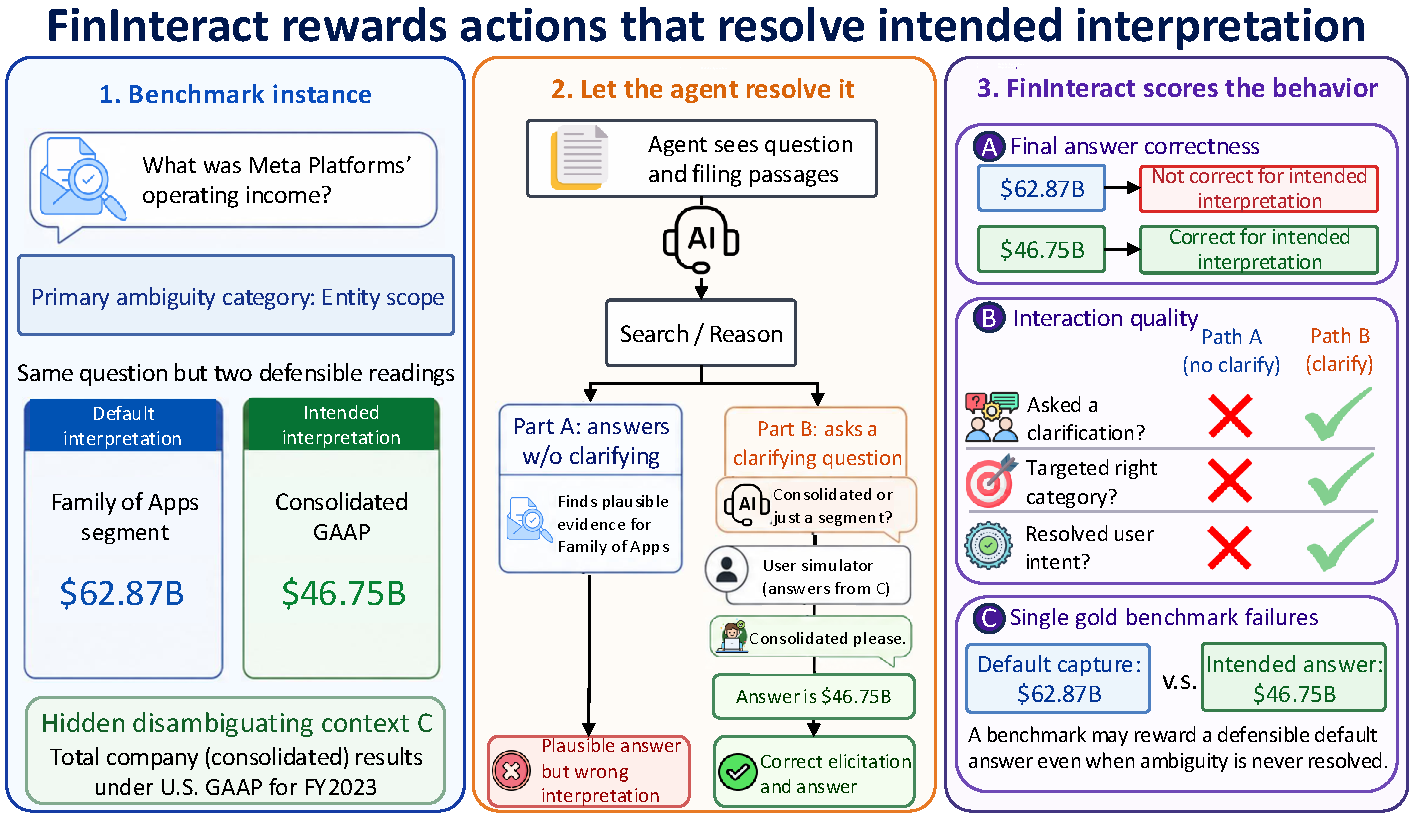
\includegraphics[width=\textwidth]{workflow_plot.pdf}
\caption{\textbf{\fininteract rewards actions that resolve the intended interpretation.}
\textbf{(1)~Benchmark instance:} the question (Meta Platforms' operating income) carries a
primary ambiguity category (entity scope) and two defensible readings, a default (Family of
Apps segment, \$62.87B) and an intended (consolidated GAAP, \$46.75B), separated by a hidden
disambiguating context $C$. \textbf{(2)~Let the agent resolve it:} seeing the question and
filing passages, the agent either answers without clarifying (Part~A, a plausible but wrong
interpretation) or asks a clarifying question that a user simulator answers only from $C$
(Part~B, correct elicitation and answer). \textbf{(3)~\fininteract scores the behavior}
on three signals: final-answer correctness against the intended interpretation, interaction
quality (did the agent ask, target the right category, and resolve the user's intent), and
the single-gold failure a conventional benchmark makes by rewarding the defensible default.}
\label{fig:framework}
\end{figure*}

\subsection{Validation}
\label{sec:humanval}
We employ finance-literate annotators, including Chartered Financial Analyst (CFA) charterholders and licensees from Hong Kong Securities and Futures Commission (SFC), to review instances to check whether 1) question $Q$ is ambiguous and 2) disambiguating context $C$ uniquely identifies the intended reading without stating the answer and 3) both intended and default answers are correct. We record a substantial agreement with an average 0.85 Gwet's AC1~\citep{gwet2008}, indicating strong chance-corrected consensus that, unlike Cohen's $\kappa$, stays reliable under the heavy skew toward ``yes'' labels. The full protocol and annotation details are in Appendix~\ref{app:construction}.

\subsection{Metrics}
\label{sec:metrics}

We deliberately lead with metrics that are standard in the ambiguous-QA and
interactive-retrieval literature (accuracy, calibration, interaction counts),
so that \fininteract is directly comparable to prior benchmarks rather than
self-referential. A single bespoke efficiency score is reported only as a
supplementary diagnostic.

\textbf{Accuracy (\%)} (primary) is the fraction of instances whose final
answer matches the \emph{intended} interpretation, graded by GPT-4o-mini with
financial-domain tolerance ($\pm$1\% numeric, entity/ticker equivalence,
currency normalization; fiscal-year mismatch = wrong). This is the metric on
which models are ranked, mirroring \interactcomp, BrowseComp, and FinanceBench.

\textbf{Default-capture rate (\%)} is the fraction whose final answer instead
matches the \emph{default} interpretation. It measures how often a model
confidently returns the naive reading, and lets us reconstruct what a
conventional single-gold benchmark would have scored (\S\ref{sec:illusion}).

\textbf{Interaction diagnostics} (secondary, descriptive): \emph{IR}
(interaction rate, \% of instances with $\geq 1$ ask), \emph{Round} (mean
turns), and \emph{CategoryHit}, for each interact action GPT-4o-mini classifies
whether the clarifying question targets a true ambiguity category for that instance;
we report CategoryHit@1, AnyCategoryHit, WrongCategoryRate, and GenericAskRate. Because
clarifications are often compound (one question can name an entity, a period, and a metric
at once), we report CategoryHit@1 in two forms: a lenient \emph{touch} form (the question names
any true category) and a strict \emph{central} form (the single most-central category is a true
category). The touch form is validated against human annotators (\S\ref{sec:humanval}). These
metrics characterize \emph{how} a model interacts and do not rank models.

\textbf{Calibration}: 5-bin Expected Calibration Error (ECE) between stated
confidence and correctness, capturing overconfidence on ambiguous queries.

\textbf{\disep (supplementary).} As a single number folding accuracy and
clarification cost together we report the efficiency of \emph{successful}
clarification,
\[
  \text{DisE}^+ = \mathbf{1}[\text{correct}] \times
  \mathbf{1}[n_\text{asks}{>}0] \times \frac{H_0}{n_\text{asks}},
\]
which is positive only when the agent asked at least one question and then
answered correctly, and decreases with redundant asks. We restrict it to the
asked-and-correct case precisely to avoid the perverse incentive of an
all-instances variant, which would award its maximum to a confident
\emph{zero-ask} answer, rewarding the very behavior the benchmark penalizes.
DisE$^+$ is a diagnostic of clarification efficiency, never the ranking metric.


%% ============================================================
\section{Experiments}
\label{sec:exp}
\label{sec:eval}
%% ============================================================
\subsection{Evaluation setup}
\textbf{Agent architecture.} We evaluate agents under the ReAct~\citep{yao2023react} framework in the seven configurations of Table~\ref{tab:modes}. The \textbf{interact} action presents a yes-or-no question to the simulated user, who must respond ``yes'', ``no'', or ``I don't know''.

\textbf{Prompting strategy.} \fininteract evaluates interactive agents under several interaction protocols: answer-only, answer with search, answer with search and interaction, and the category-conditioned policies. All models run under the same ReAct system prompt. Additional details are in Appendix~\ref{sec:error}.

\textbf{Models.} We evaluate a diverse set of models. The proprietary set comprises the GPT family (GPT-5.6, GPT-5, GPT-4o, and GPT-5-mini), Claude-Sonnet-5, Gemini-3.5-flash, Grok-4.5, DeepSeek-V4-flash, GLM-5.2, and Kimi-K3. The open-source set comprises the dense Qwen3 family (4B, 8B, 14B, and 32B) and two mixture-of-experts models, Qwen3-30B-A3B and Qwen3.5-35B-A3B. Proprietary models are accessed through a unified OpenRouter harness.

\subsection{Overall performance}
\label{sec:ceiling}
Even frontier models are vulnerable to financial report ambiguity (Table~\ref{tab:main}). No model exceeds $44\%$ accuracy on the intended interpretation under free interaction, and the ceiling is low for proprietary and open-source models alike: the best full-scale model reaches $28.9\%$ and the best cross-vendor pilot model $44.0\%$.

The opportunity to interact does not by itself improve accuracy. The interaction difference $\Delta$ (added-interaction minus plain-search accuracy) is non-positive for eleven of the sixteen evaluated models, so the failure is not one of asking but of converting a clarified intention into the correct answer. For the three proprietary models we run with full interaction diagnostics this reading is direct: they interact on $96$--$99\%$ of instances and target a true ambiguity category at AC@1 $0.86$--$0.94$, so they do recognize which kind of ambiguity is present and do ask about it, yet still answer wrongly. The open models interact far less often ($15$--$72\%$), so their negative $\Delta$ mixes under-asking with the same integration failure.

Two ablations bracket this gap (Table~\ref{tab:ceiling}). Forcing four rounds of clarification \emph{lowers} accuracy rather than raising it, which is consistent with agents getting lost in multi-turn conversations~\citep{laban2026llms}. Supplying the disambiguating context $C$ as an oracle instead lifts every model to $93$--$95\%$. Because $C$ never contains the final answer $A$, this improvement shows that the gap is not missing knowledge but the ability to resolve the interpretation and carry it into the answer. Appendix~\ref{app:maindetails} reports the full analysis. \textbf{Finding 1: models can observe the ambiguity and answer correctly once the intention is made explicit, but fail to bridge the intermediate step from an updated intention to the correct answer.}

\begin{table}[t]
\centering
\caption{Forcing more clarification does not help accuracy, but \emph{resolving} the ambiguity lifts every model to $93$--$95\%$. The gap is therefore the model's inability to elicit $C$ for itself, not missing knowledge or grounding. Abbreviations follow Table~\ref{tab:modes}.}
\label{tab:ceiling}
\small
\begin{tabular}{lcccc}
\toprule
Model & A & A+I & Forced(4) & \textbf{Oracle} \\
\midrule
GPT-5      & 0.6 & 20.2 & 1.5 & \textbf{95.4} \\
GPT-4o     & 0.6 & 4.6  & 0.0 & \textbf{93.1} \\
GPT-5-mini & 0.6 & 0.0  & 0.6 & \textbf{95.4} \\
Qwen3-30B   & 1.2 & 11.6 & -- & \textbf{90.2} \\
Qwen3.5-35B & 0.6 & 28.9 & -- & \textbf{91.9} \\
\bottomrule
\end{tabular}
\end{table}

\newlength{\midgap}\setlength{\midgap}{-0.02\textwidth}% <-- gap between the two panels; adjust here
\begin{table*}[t]
\centering
\caption{\textbf{(a)}~Main results, reporting accuracy (\%) against the \emph{intended}
interpretation per mode, with $\Delta$ the +Interact minus +Search difference (full-scale rows are
$N{=}173$ and the cross-vendor frontier rows, IR and ECE blank, are a preliminary $N{=}50$ pilot).
\textbf{(b)}~Re-grading the same outputs against the intended versus the default reading a conventional benchmark would treat as gold (Same abbreviation as Table~\ref{tab:modes}). \textbf{(c)}~Per-category targeting
(AC@1), where recognition policy is a shared blind spot ($=0$ for every model). Category
sizes: entity (Ent.) 94, metric (Met.) 63, recognition (Rec.) 9, temporal (Tmp.) 7.}
\label{tab:main}
%
\begin{minipage}[t]{0.57\textwidth}
\centering
\textbf{(a) Main results}\par\smallskip
{\small\setlength{\tabcolsep}{2.5pt}
\begin{tabular}{lccccccc}
\toprule
& \multicolumn{2}{c}{Acc (\%)} &
  \multicolumn{5}{c}{Answer+Search+Interact} \\
\cmidrule(lr){2-3}\cmidrule(lr){4-8}
Model & A & A+S & A+S & $\Delta$ & IR & AC@1 & ECE \\
\midrule
\multicolumn{8}{l}{\textit{Proprietary models}} \\
GPT-5.6           & 10.0 & 36.0 & 30.0 & $-6$  & -- & .98 & -- \\
GPT-5             & 0.6 & 6.4  & \textbf{20.2} & $+13.8$ & 98.8 & .86 & .53 \\
GPT-4o            & 0.6 & 12.1 & 4.6  & $-7.5$  & 99.4 & .94 & .82 \\
GPT-5-mini        & 0.6 & 0.0  & 0.0  & $0.0$   & 96.0 & .94 & .00 \\
Claude-Sonnet-5   & 4.0  & \textbf{46.0} & \textbf{44.0} & $-2$  & -- & .98 & -- \\
Grok-4.5          & 2.0  & 40.0 & 32.0 & $-8$  & -- & .87 & -- \\
GLM-5.2           & 12.0 & 40.0 & 40.0 & $0$   & -- & .96 & -- \\
Kimi-K3           & 16.0 & 38.0 & 34.0 & $-4$  & -- & .98 & -- \\
DeepSeek-V4-flash & 12.0 & 28.0 & 24.0 & $-4$  & -- & .96 & -- \\
Gemini-3.5-flash  & 14.0 & 6.0  & 30.0 & $+24$ & -- & .96 & -- \\
\midrule
\multicolumn{8}{l}{\textit{Open source models}} \\
Qwen3-4B          & 0.0 & 8.1  & 12.1 & $+4.0$  & 28 & .85 & -- \\
Qwen3-8B          & 0.6 & 14.4 & 24.9 & $+10.5$ & 15 & .88 & -- \\
Qwen3-14B         & 0.0 & 18.5 & 22.5 & $+4.0$  & 36 & .74 & -- \\
Qwen3-32B         & 1.2 & 27.2 & 8.4  & $-18.8$ & 61 & .96 & -- \\
Qwen3-30B-A3B     & 1.2 & 28.3 & 11.6 & $-16.7$ & 72 & .90 & -- \\
Qwen3.5-35B-A3B   & 0.6 & \textbf{35.8} & 28.9 & $-6.9$ & 36 & .81 & -- \\
\midrule
\multicolumn{8}{l}{\textit{Human baseline ($N{=}50$)}} \\
Human             & -- & -- & \textbf{30.0} & -- & 100 & .72 & -- \\
\bottomrule
\end{tabular}}
\end{minipage}\hspace{\midgap}%
\begin{minipage}[t]{0.45\textwidth}
\centering
\textbf{(b) Single-gold illusion}\par\smallskip
{\small
\begin{tabular}{p{1cm}lccc}
\toprule
Model & Mode & Intended & Default & $\Delta$ \\
      &      & (true Acc) & (single-gold) & \\
\midrule
\multirow{3}{1cm}{GPT-5}  & A   & 0.6  & 2.3  & +1.7 \\
       & A+S & 6.4  & 10.4 & +4.0 \\
       & A+S+I & \textbf{20.2} & 12.1 & $-8.1$ \\
\midrule
\multirow{3}{1cm}{GPT-4o} & A & 0.6  & 0.6  & 0.0 \\
       & A+S & 12.1 & \textbf{37.0} & \textbf{+24.9} \\
       & A+S+I & 4.6  & 6.4  & +1.8 \\
\midrule
\multirow{3}{1cm}{GPT-5-mini} & A & 0.6 & 0.0 & $-0.6$ \\
           & A+S & 0.0 & 0.0 & 0.0 \\
           & A+S+I & 0.0 & 0.0 & 0.0 \\
\bottomrule
\end{tabular}}
\par\bigskip
\textbf{(c) Per-category targeting (AC@1)}\par\smallskip
{\small
\begin{tabular}{lcccc}
\toprule
Model & Ent. & Met. & Rec. & Tmp. \\
\midrule
GPT-5    & .89 & .92 & \textbf{.00} & 1.00 \\
GPT-4o   & 1.00 & .97 & \textbf{.00} & 1.00 \\
GPT-5-m  & .99 & 1.00 & \textbf{.00} & 1.00 \\
Q3-30B   & .93 & .96 & \textbf{.00} & 1.00 \\
Q3.5-35B & .85 & .87 & \textbf{.00} & 1.00 \\
\bottomrule
\end{tabular}}
\end{minipage}
\end{table*}


\subsection{Failure of existing benchmarks}
\label{sec:illusion}

Because every instance carries both a default and an intended answer, we can re-grade the \emph{identical} model outputs under the two conventions and read off what a conventional single-gold benchmark would have reported (Table~\ref{tab:main}(b)). In the retrieval-augmented regime where such benchmarks operate, grading against the default inflates the score sharply: GPT-4o is credited $37.0\%$ against the default but only $12.1\%$ against the intended reading, so a single-gold benchmark would have reported $3.1\times$ its true competence. The inflation reverses only under interaction, where GPT-5 scores $20.2\%$ intended against $12.1\%$ default, which is precisely the point: asking is what converts a default-anchored guess into the intended answer, and it is the one behavior single-gold grading cannot see. Appendix~\ref{app:maindetails} reports the full re-grading together with a human study confirming that annotators shown only $Q$ and the passage record the default reading as gold $66\%$ of the time. \textbf{Finding 2: a single-gold convention overstates competence by up to $3.1\times$, because one gold answer per question encodes the default reading rather than the intended one.}



\subsection{Targeting varies by ambiguity category}
\label{sec:skills}
Aggregate AC@1 hides where clarification actually succeeds, so we decompose targeting by ambiguity category (Table~\ref{tab:main}(c)). Models name the correct category almost always for entity scope, metric definition, and temporal scope, but never for recognition policy, where AC@1 is $0$ for every model evaluated. A case study makes the missed distinction concrete. Asked ``What were General Electric's revenues?'', a model may answer \$67.95B or \$26.79B depending on the recognition basis: the former is GAAP revenue combining over-time service recognition with point-in-time product recognition, the latter counts only revenue recognized at a point in time. Models return a single figure without asking which basis is meant, defaulting to the assumption that ``revenue'' is well defined and passing over the ASC~606 distinction between point-in-time and over-time recognition. We read this as evidence that a domain-specific reporting practice is not reflected in current models' general clarification behavior, which is what motivates the category-conditioned interventions of Sec.~\ref{sec:trainsignal}.

This last observation carries an important caveat. Recognition policy is one of our three exploratory categories, with only $n{=}9$ instances, and an item-level audit (Appendix~\ref{app:limitations}) finds most of them to be ASC~606 timing disaggregations where neither value is the total a non-expert would assume. Our two human annotators also never targeted the category, so the blind spot is at least not model-specific. We therefore report it as a preliminary observation on a small sample rather than a quantitative result, and treat entity scope ($n{=}94$) and metric definition ($n{=}63$) as the two well-powered categories. \textbf{Finding 3: targeting accuracy is uneven across ambiguity categories; entity, metric, and temporal ambiguity are reliably named, while recognition policy is never raised, on preliminary evidence from a nine-instance category.}

\subsection{Ambiguity category as training signal}
\label{sec:trainsignal}
The diagnosis so far is descriptive, so we ask whether the ambiguity category can also serve as a training signal. We run category-conditioned training on a Qwen3-4B policy, supervised fine-tuning on category-guided demonstrations followed by reinforcement learning, teaching the model to interact and to target the correct category. On the held-out split the leak-proof signals rise almost entirely at the supervised stage, with AC@1 going from $25$ to $69$ and interaction from $55$ to $100$ (Table~\ref{tab:grpo}, Figure~\ref{fig:grpo}a), while the later stages move within run-to-run noise at $n{=}51$. Full multi-turn reinforcement learning confirms that the episode is trainable end to end, with clarifying turns rising from $5.7$ to $8.6$ (Figure~\ref{fig:grpo}b). At inference time the same idea, conditioning on the category, lifts GPT-5 from $34.0\%$ to $46.0\%$ on a stratified $N{=}50$ pilot (Appendix~\ref{sec:axisreact}). The gains concentrate on the data-abundant categories, so the signal is actionable but does not reach the recognition-policy blind spot of Sec.~\ref{sec:skills}. Additional details are in Appendix~\ref{sec:grpo}. \textbf{Finding 4: conditioning on the ambiguity category improves clarification at both training and inference time, so \fininteract provides an actionable signal and not only a diagnosis.}

\begin{table}[t]
\centering
\caption{RLVR ladder on \fininteract with Qwen3-4B, held-out $n{=}51$. Category-guided supervision installs on-category clarification, with the leak-proof signals (AC@1 and interaction) rising almost entirely at the SFT stage. Accuracy is leak-confounded and is reported for completeness only.}
\label{tab:grpo}
\small
\begin{tabular}{lcccc}
\toprule
Stage & AC@1 & Interaction & Accuracy & Reward \\
\midrule
Base      & 25.0 & 54.9 & 84.3 & 0.96 \\
\;\;+\,SFT & 68.6 & \textbf{100} & 88.2 & 1.28 \\
\;\;+\,KTO               & \textbf{70.6} & \textbf{100} & 84.3 & 1.27 \\
\;\;+\,GRPO              & 66.7 & \textbf{100} & 88.2 & \textbf{1.30} \\
\bottomrule
\end{tabular}
\end{table}

\begin{figure*}[t]
\centering
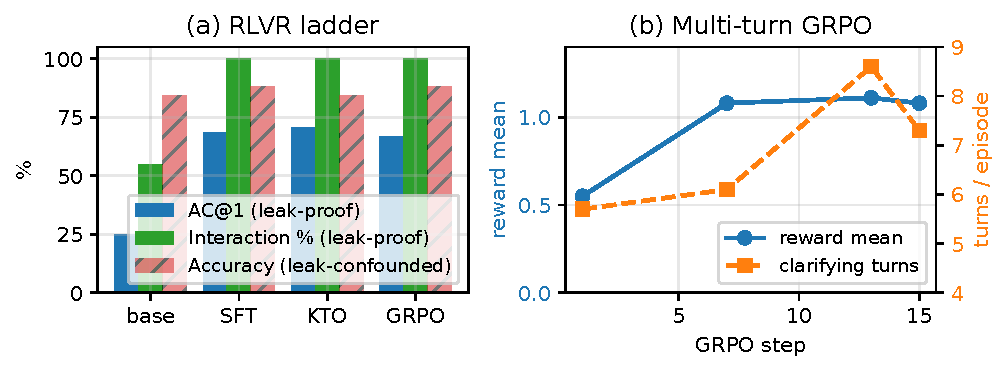
\includegraphics[width=0.9\textwidth]{fig_grpo_insights.pdf}
\caption{\textbf{Category-guided training installs on-category clarification.} (a) The leak-proof signals, AC@1 and interaction rate, jump at the supervised stage and change little thereafter. (b) True multi-turn GRPO on the 4B policy: mean reward and clarifying turns rise together over training.}
\label{fig:grpo}
\end{figure*}

%% ============================================================
\section{Discussion}
\label{sec:discussion}
%% ============================================================
We draw four takeaways here and develop each in Appendix~\ref{app:discussion}. \textbf{Ambiguity categories are different learning problems}, so an aggregate interaction score hides where the difficulty actually sits. \textbf{Elicitation is a trainable skill that current models lack}, so progress depends less on larger backbones than on objectives that reward asking about the right category at the right time. \textbf{Ambiguity persists in human-AI collaboration}, since models confidently return the default reading even with domain experts in the loop. \textbf{The paired construction should transfer to further categories, languages, and high-stakes domains}, wherever a single gold answer hides genuine ambiguity.


%% ============================================================
\section{Related Work}
\label{sec:related}
%% ============================================================
We include the most relevant works to \fininteract and defer additional financial and general-domain benchmarks as well as more widespread related work in Appendix~\ref{app:related}.
%% ============================================================

\textbf{Financial QA benchmarks} such as FinanceBench~\citep{islam2023financebench}, FinQA~\citep{chen2021finqa}, and DocFinQA~\citep{reddy2024docfinqa}, together with recent agentic successors, enforce single-gold, single-turn evaluation and test numerical reasoning or retrieval without exploring whether a query is under-specified. To our knowledge, \fininteract is the first to make query ambiguity the central focus through paired default/intended interpretations and multi-turn interaction in the financial domain. We include comparison with existing financial QA benchmarks in Appendix~\ref{app:related}.

\textbf{Ambiguous QA and clarifying questions.} In the general domain, AmbigQA~\citep{min2020ambigqa}, CLAMBER~\citep{zhang2024clamber}, and QuestBench~\citep{li2025questbench} study whether a model identifies under-specification and asks the minimal clarifying question, building on a long clarifying-question line in retrieval and dialogue. \interactcomp~\citep{interactcomp2026} is our direct methodological ancestor, which we extend to finance with a domain-specific ambiguity taxonomy, per-category targeting (AC@1), and programmatically verifiable XBRL-grounded evidence pairs.

\textbf{Multi-turn interaction and selective answering.} Large models often \emph{lose track} over multi-turn conversations~\citep{laban2026llms}, and calibrated systems frequently do better by answering \emph{selectively} or abstaining under ambiguity~\citep{cole2023selectively,kuhn2022clam}. Our findings echo this in the financial setting, where forcing extra clarification degrades accuracy, but \fininteract turns the observation into a controlled, per-category diagnosis of \emph{which} clarification an agent should issue and \emph{whether} issuing it resolves the query, instead of only measuring whether more turns help.

%% ============================================================
\section{Conclusion}
\label{sec:conclusion}
%% ============================================================
We introduced \fininteract, to our knowledge the first bilingual benchmark that evaluates financial search agents on genuinely ambiguous queries. Its five-category ambiguity taxonomy, paired default and intended interpretation design, and construction pipeline with an adversarial verifier yield 173 instances that resist trivial disambiguation. Our central finding is that the bottleneck in handling financial QA ambiguity is interaction capability rather than financial knowledge, and that this capability has two parts: asking for the right clarification, and updating the answer once the clarification arrives. When the ambiguity is resolved for them, agents answer at 93-95\% accuracy, against at most 28.9\% when they must elicit the resolution themselves. This extends the interaction stagnation identified in \interactcomp to a domain whose terminology is far more specific, and where the cost of a confident wrong answer is correspondingly higher. We further turn the diagnosis into an intervention in Sec.~\ref{sec:trainsignal}, showing that \fininteract also serves as an informative training signal, and we release it with full construction, evaluation, and training code for reproducible follow-on work.


%% ============================================================
%% ARR CFP: Limitations is REQUIRED, unnumbered, placed after the conclusion
%% and before the references, and "it will not count toward the page limit".
%% Long papers get 8 pages of content plus unlimited extra space for this
%% section and for an optional ethics section, plus unlimited references.
%% Appendices come after the references and also do not count.
%% (The bundled formatting.md does not state this; it defers to the venue CFP.)
%% ============================================================
\section*{Limitations}
%% Shared by main.tex (inside the Discussion section, AAAI) and by
%% main_acl.tex (as the unnumbered \section*{Limitations} that *ACL requires).
We note the following limitations of this study.
\begin{enumerate}[leftmargin=*,itemsep=1pt,topsep=3pt]
  \item \textbf{Scale.} A 173-instance corpus is small, a consequence of prioritizing per-instance construction rigor.
  \item \textbf{Language balance.} The English-to-Chinese split is 53:120, which may favor models pre-trained more heavily in one of the two languages.
  \item \textbf{Dominating categories.} Entity scope (n = 94) and metric definition (n = 63) dominate, against only n = 9 for recognition policy, which suggests that current models are not able to generate instances of the rarer categories in the first place.
  \item \textbf{Generator and evaluator bias.} Under API budget constraints we use the GPT-5 family for construction and simulation, which may bias results toward that family.
  \item \textbf{Data contamination.} Instances are freshly constructed from FY2022-2025 facts, but we cannot rule out that recently released models were pre-trained on those filings.
\end{enumerate}
Appendix~\ref{app:limitations} expands each of these.


%% ============================================================
%% Optional per the ARR CFP, and likewise exempt from the page limit when
%% placed at the end. Answers item A1 of the Responsible NLP checklist.
%% ============================================================
\section*{Ethical Considerations}
%% Unnumbered "Ethical Considerations" section. *ACL exempts it from the page
%% limit when placed after the conclusion, so it is inputted only by
%% main_acl.tex; the AAAI build has no such exemption.
\textbf{Deployment risk is the motivation and also the hazard.} The agents we study feed
financial analytics and investment decisions, and our central result is that they commit
confidently to an unintended reading of an ambiguous question far more often than they ask.
A wrong number produced this way is well grounded in a real filing, so it is unusually hard
for a downstream user to catch. We therefore frame the benchmark as a reason to prefer
systems that ask and abstain over systems that answer, and we caution that a high score on
\fininteract measures a narrow clarification ability, not readiness for deployment in a
setting where a confident wrong figure carries financial consequences.

\textbf{Intended use and misuse.} \fininteract is an evaluation resource, not a training
corpus and not financial advice, as stated in its datasheet (Appendix~\ref{app:datasheet}).
Because every instance is ambiguous by construction, the benchmark does not measure a
calibrated decision of \emph{when} to ask, so it should not be used to certify that a system
asks appropriately in general deployment; we make this limitation explicit in
Appendix~\ref{app:limitations}.

\textbf{Data provenance and privacy.} All source documents are public regulatory filings:
SEC EDGAR filings for the English split and CSRC annual reports retrieved via CNINFO and
akshare for the Chinese split. No proprietary, paywalled, or personal data is used. Instances
consist of questions about corporate financial metrics and carry company identifiers rather
than individuals, so the released artifact contains no personally identifying information and
no objectionable content. Third-party corpora used only during construction are not
redistributed.

\textbf{Compute and environmental cost.} The evaluation is API-based rather than
training-heavy. We instrument and report the full construction cost in
Appendix~\ref{app:cost}, at \$0.31 per accepted instance and about \$54 for the released
corpus. The only model training in this work is 4-bit QLoRA on a 4B-parameter policy, run for
tens of optimization steps rather than to convergence, so the associated energy cost is small
relative to a typical pretraining or full fine-tuning study.


%% ============================================================
%% acl.sty sets \bibliographystyle{acl_natbib}; do not set it again.
%% ============================================================
\bibliography{refs}

\appendix
\input{paper/sections/appendix}

\end{document}
